% Copyright (C) 2010,2011,2012,2013,2014,2015,2016 The ESPResSo project
% Copyright (C) 2002,2003,2004,2005,2006,2007,2008,2009,2010 
%   Max-Planck-Institute for Polymer Research, Theory Group
%  
% This file is part of ESPResSo.
%   
% ESPResSo is free software: you can redistribute it and/or modify it
% under the terms of the GNU General Public License as published by the
% Free Software Foundation, either version 3 of the License, or (at your
% option) any later version.
%  
% ESPResSo is distributed in the hope that it will be useful, but
% WITHOUT ANY WARRANTY; without even the implied warranty of
% MERCHANTABILITY or FITNESS FOR A PARTICULAR PURPOSE.  See the GNU
% General Public License for more details.
%  
% You should have received a copy of the GNU General Public License
% along with this program.  If not, see <http://www.gnu.org/licenses/>.
%
\chapter{Getting, compiling and running \es}
\label{chap:install}
\index{Installation|textbf}

This chapter will describe how to get, compile and run the \es
software.  

\es releases are available as source code packages from the \es home
page\footnote{\url{http://espressomd.org}}.  This is where new users
should get the code.  The code within release packages is tested and
known to run on a number of platforms.  Alternatively, people that
want to use the newest features of \es or that want to start
contributing to the software can instead obtain the current
development code via the version control system software
\textsf{git}\footnote{\url{http://git.org}} from \es's project page at
Github \footnote{\url{https://github.com/espressomd/espresso}}.
This code might be not as well tested and documented as the release
code; it is recommended to use this code only if you have already
gained some experience in using \es.

Unlike most other software, no binary distributions of \es are
available, and the software is usually not installed globally for all
users.  Instead, users of \es should compile the software themselves.
\index{features} The reason for this is that it is possible to
activate and deactivate various features before compiling the code.
Some of these features are not compatible with each other, and some of
the features have a profound impact on the performance of the code.
Therefore it is not possible to build a single binary that can satisfy
all needs.  F or performance reasons a user should always activate only those features that are
actually needed.  This means, however, that learning how to compile
\es is a necessary evil.  
The build system of \es uses either the GNU
autotools or cmake to
compile software easily on a wide range of platforms.

\section{cmake}
In order to build \es the first step is to create a build directory in which cmake can be executed. In cmake, the \emph{source directory} (that contains all the source
files) is completely separated from the \emph{build directory} (where the files created by the build process are put). cmake is designed to not be executed in the source directory.
Cmake will determine how to use and where to find
the compiler, as well as the different libraries and tools required by
the compilation process. By having multiple build directories you can build several
variants of \es, each variant having different activated features, and
for as many platforms as you want.

\paragraph{Example}
When the source directory is \codebox{srcdir} (\ie the files where
unpacked to this directory), then the user can create a build directory
\codebox{build} below that path by calling the \codebox{mkdir srcdir/build}. In the build directory cmake is to be executed, followed by a call of make. None of the files in the source directory is ever modified when by the build process.
\begin{code}
cd build
cmake srcdir
make
Espresso
\end{code}
Afterwards Espresso can be run via calling Espresso from the command line.
\subsection{ccmake}
Optionally and for easier use the curses interface to cmake can be used to configure ESPResSo interactively. 
\paragraph{Example}
Alternatively to the previous example instead of \codebox{cmake}, the \codebox{ccmake} executable is called in the build directory to configure ESPResSo previous to its compilation followed by a call of make:
\begin{code}
cd build
ccmake srcdir
make
Espresso
\end{code}
Fig.~\ref{fig:ccmake} shows the interactive ccmake UI.
\begin{figure}[tb]
  \centering
  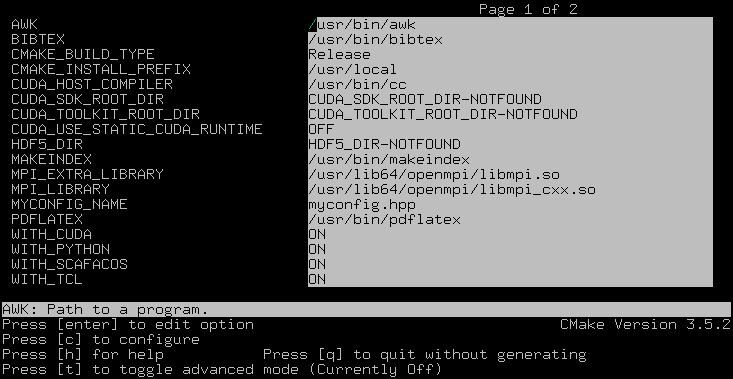
\includegraphics[width=0.7\textwidth]{figures/ccmake-example.png}
  \caption{ccmake interface}
  \label{fig:ccmake}
\end{figure}


\subsection{Options and Variables}
The behavior of \codebox{cmake} can be
controlled by the means of options and variables in the CMakeLists.txt file. Also options are defined there.
The following options are available:
\begin{description}
	\item WITH_PYTHON: Build python interface
	\item WITH_TCL: Build tcl interface
	\item WITH_CUDA: Build with GPU support
        \item WITH_HDF5: Build with HDF5
	\item WITH_TESTS: Enable tests
	\item WITH_SCAFACOS: Build with Scafacos support
	\item WITH_VALGRIND_INSTRUMENTATION: Build with valgrind instrumentation markers
\end{description}
When the value in the CMakeLists.txt file is set to ON the corresponding option is created if the value of the option is set to OFF the corresponding option is not created. 
These options can also be modified by calling cmake with the command line argument -D:
\begin{code}
cmake -D WITH_TCL=OFF srcdir 
\end{code}
In the rare event when working with cmake and you want to have a totally clean build (for example because you switched the compiler), remove the build directory and create a new one.
\section{\texttt{make}: Compiling,  testing and installing \es}
\label{sec:make}

The command \texttt{make} is mainly used to compile the \es source
code, but it can do a number of other things. The generic syntax of
the \texttt{make} command is:
\begin{code}
make [\var{options}] [\var{target}...] [\var{variable}=\var{value}]
\end{code}
When no target is given, the target \texttt{all} is used. The
following targets are available:
\begin{description}
\item[\texttt{all}] Compiles the complete \es source code. The
  variable \lit{myconf} can be used to specify the name of the
  configuration header to be used.
\item[\texttt{check}] Runs the testsuite. By default, all available
  tests will be run on 1, 2, 3, 4, 6, or 8 processors. Which tests are
  run can be controlled by means of the variable \texttt{tests}, which
  processor numbers are to be used can be controlled via the variable
  \texttt{processors}. Note that depending on your MPI installation,
  MPI jobs can only be run in the queuing system, so that \es{} will
  not run from the command line. In that case, you may not be able to
  run the testsuite, or you have to directly submit the testsuite script
  \verb!testsuite/test.sh! to the queuing system.\\
  \textbf{Example:} \verb!make check tests="madelung.tcl" processors="1 2"!\\
  will run the test \texttt{madlung.tcl} on one and two processors.
\item[\texttt{clean}] Deletes all files that were created during the
  compilation.
\item[\texttt{mostlyclean}] Deletes most files that were created
  during the compilation. Will keep for example the built doxygen
  documentation and the \es{} binary.
\item[\texttt{dist}] Creates a \texttt{.tar.gz}-file of the \es{}
  sources.  This will include all source files as they currently are
  in the source directory, \ie{} it will include local changes.  This
  is useful to give your version of \es{} to other people.
  The variable \texttt{extra} can be used to specify additional
  files and directories that are to be included in the archive
  file. \\
  \textbf{Example:} \verb!make dist extra="myconfig.hpp internal"!\\
  will create the archive file and include the file
  \texttt{myconfig.hpp} and the directory \texttt{internal} with all
  files and subdirectories.
\item[\texttt{install}] Install \es. The variables \texttt{prefix} and
  \texttt{exec-prefix} can be used to specify the installation
  directories, otherwise the defaults defined by the
  \texttt{configure} script are used. \texttt{prefix} sets the prefix
  where all \es files are to be installed, \texttt{exec-prefix} sets
  the prefix where the executable files are to be installed and is
  required only when there is an architecture-specific directory.\\
  \textbf{Example:} \verb!make install prefix=/usr/local!\\
  will install all files below \texttt{/usr/local}.
\item[\texttt{ug\ \ }] Creates the User guide in the \texttt{doc/ug}
  subdirectory (only when using the development sources).
\item[\texttt{dg\ \ }] Creates the Developers' guide in the
  \texttt{doc/dg} subdirectory (only when using the development
  sources).
\item[\texttt{doxygen\ \ }] Creates the Doxygen code documentation in the
  \texttt{doc/doxygen} subdirectory.
\item[\texttt{tutorials\ \ }] Creates the \es tutorials in the
  \texttt{doc/tutorials} subdirectory.
\item[\texttt{doc\ }] Creates all documentation in the \texttt{doc}
  subdirectory (only when using the development sources).
\end{description}

A number of options are available when calling \texttt{make}.  The
most interesting option is probably \texttt{-j \textit{num\_jobs}},
which can be used for parallel compilation on computers that have more
than one CPU or core.  \textit{num\_jobs} specifies the maximal number
of jobs that will be run.  Setting \textit{num\_jobs} to the number of
available processors speeds up the compilation process significantly.

\section{TCL: Running \es}
\label{sec:run}

When \es is found in your path, it can be run via
\begin{code}
Espresso [\var{tcl\_script} [\var{args}]]
\end{code}

\index{interactive mode} When \es{} is called without any arguments,
it is started in the interactive mode, where new commands can be
entered on the command line. When the name of a \textit{tcl\_script}
is given, the script is executed. Any further arguments are passed to
the script.

If you want to run \es in parallel using MPI, the actual invocation
depends on your MPI implementation. In many cases, \eg OpenMPI, the
command will be
\begin{code}
mpiexec -n \var{n\_nodes} Espresso [\var{tcl\_script} [\var{args}]]
\end{code}
where \var{n\_nodes} denotes the number of MPI nodes to be used.
However, note that depending on your MPI installation, MPI jobs can
only be run in a queuing system, so that \es will not run from the
command line. Also, older installations sometimes require ``-np''
instead of ``-n'' or ``mpirun'' instead of ``mpiexec''. 


\section{\texttt{myconfig.hpp}: Activating and deactivating features}
\label{sec:myconfig}

\index{features} \index{myconfig.hpp} \index{configuration header} \es
has a large number of features that can be compiled into the binary.
However, it is not recommended to actually compile in all possible
features, as this will slow down \es significantly.  Instead, compile
in only the features that are actually required.  A strong gain in
speed can be achieved, by disabling all non-bonded interactions except
for a single one, e.g. \feature{LENNARD_JONES}.  For the developers,
it is also possible to turn on or off a number of debugging messages.
The features and debug messages can be controlled via a configuration
header file that contains C-preprocessor declarations.  Appendix
\vref{chap:features} lists and describes all available features.  The
file \texttt{myconfig-sample.hpp} that configure will generate in the
build directory contains a list of all possible features that can be
copied into your own configuration file.  When no configuration header
is provided by the user, a default header, found in
\texttt{src/core/myconfig-default.hpp}, will be used that turns on the
default features.

When you distinguish between the build and the source directory, the
configuration header can be put in either of these. Note, however,
that when a configuration header is found in both directories, the one
in the build directory will be used.

By default, the configuration header is called \texttt{myconfig.hpp}.
The name of the configuration header can be changed either when the
\texttt{configure}-script is called via the variable
\mbox{\texttt{MYCONFIG}} (see section \vref{sec:configure}), or when
\texttt{make} is called with the setting
\mbox{\texttt{myconfig=}\textit{myconfig\_header}} (see section
\vref{sec:make}).

The configuration header can be used to compile different binary
versions of \es with a different set of features from the same source
directory.  Suppose that you have a source directory \texttt{\$srcdir}
and two build directories \texttt{\$builddir1} and
\texttt{\$builddir2} that contain different configuration headers:

\begin{itemize}
\item \texttt{\$builddir1/myconfig.hpp}:
\begin{code}
#define ELECTROSTATICS
#define LENNARD-JONES
\end{code}

\item \texttt{\$builddir2/myconfig.hpp}:
\begin{code}
#define LJCOS
\end{code}
\end{itemize}

\noindent Then you can simply compile two different versions of \es via
\begin{code}
cd $builddir1
$srcdir/configure
make

cd $builddir2
$srcdir/configure
make
\end{code}


%%% Local Variables: 
%%% mode: latex
%%% TeX-master: "ug"
%%% End: 
